\chapter{2048と強化学習}
\label{chap:rl}
完全解析はゲームの"答え"を知ることであり, 多くのプレイヤの関心の対象である.
一方で$4\times4$盤面の2048を完全解析することは難しく, 
本章では強化学習について説明する.

\section{強化学習の概要}
\label{sec:rl_general}
まず本節では2048との関係を踏まえつつ, 一般的な強化学習の概要について記述する.
なお全体に文献~\cite{Sutton1998}を参照して書かれた.

\subsection{マルコフ決定過程}
\label{subsec:mdp}
強化学習はエージェントが与えられた環境において獲得する報酬を最大化するための手法である.
強化学習が扱う問題はマルコフ決定過程~(MDP)~という枠組みによって抽象化できる. 
MDPは以下の4つの要素で構成される. 状態集合と行動集合が有限であるとき有限MDPと呼ぶ.
\begin{itemize}
  \item 状態集合\textit{S}
  \item 行動集合\textit{A}
  \item 状態遷移関数$p:S \times A \times S \rightarrow [0,1]$
  \item 報酬関数$r:S \times A \times S \rightarrow \mathbb{R}$
\end{itemize}
エージェントは時刻tで状態$s_t \in S$から行動$a_t \in A$を選択する.
そして確率$p(s_{t+1}|s_t,a_t)$で次の状態$s_{t+1}$に遷移し, 即時報酬$R_{t+1}=r(s_t,a_t,s_{t+1})$を獲得する.
エージェントが状態から行動を選択する際の確率分布$\pi:S \times A \rightarrow [0,1]$を方策という. 
また状態遷移関数と報酬関数は環境のダイナミクスと呼ばれることがある. 
図\ref{fig:mdp}にMDPの模式図を示す.

\begin{figure}[h]
  \centering
  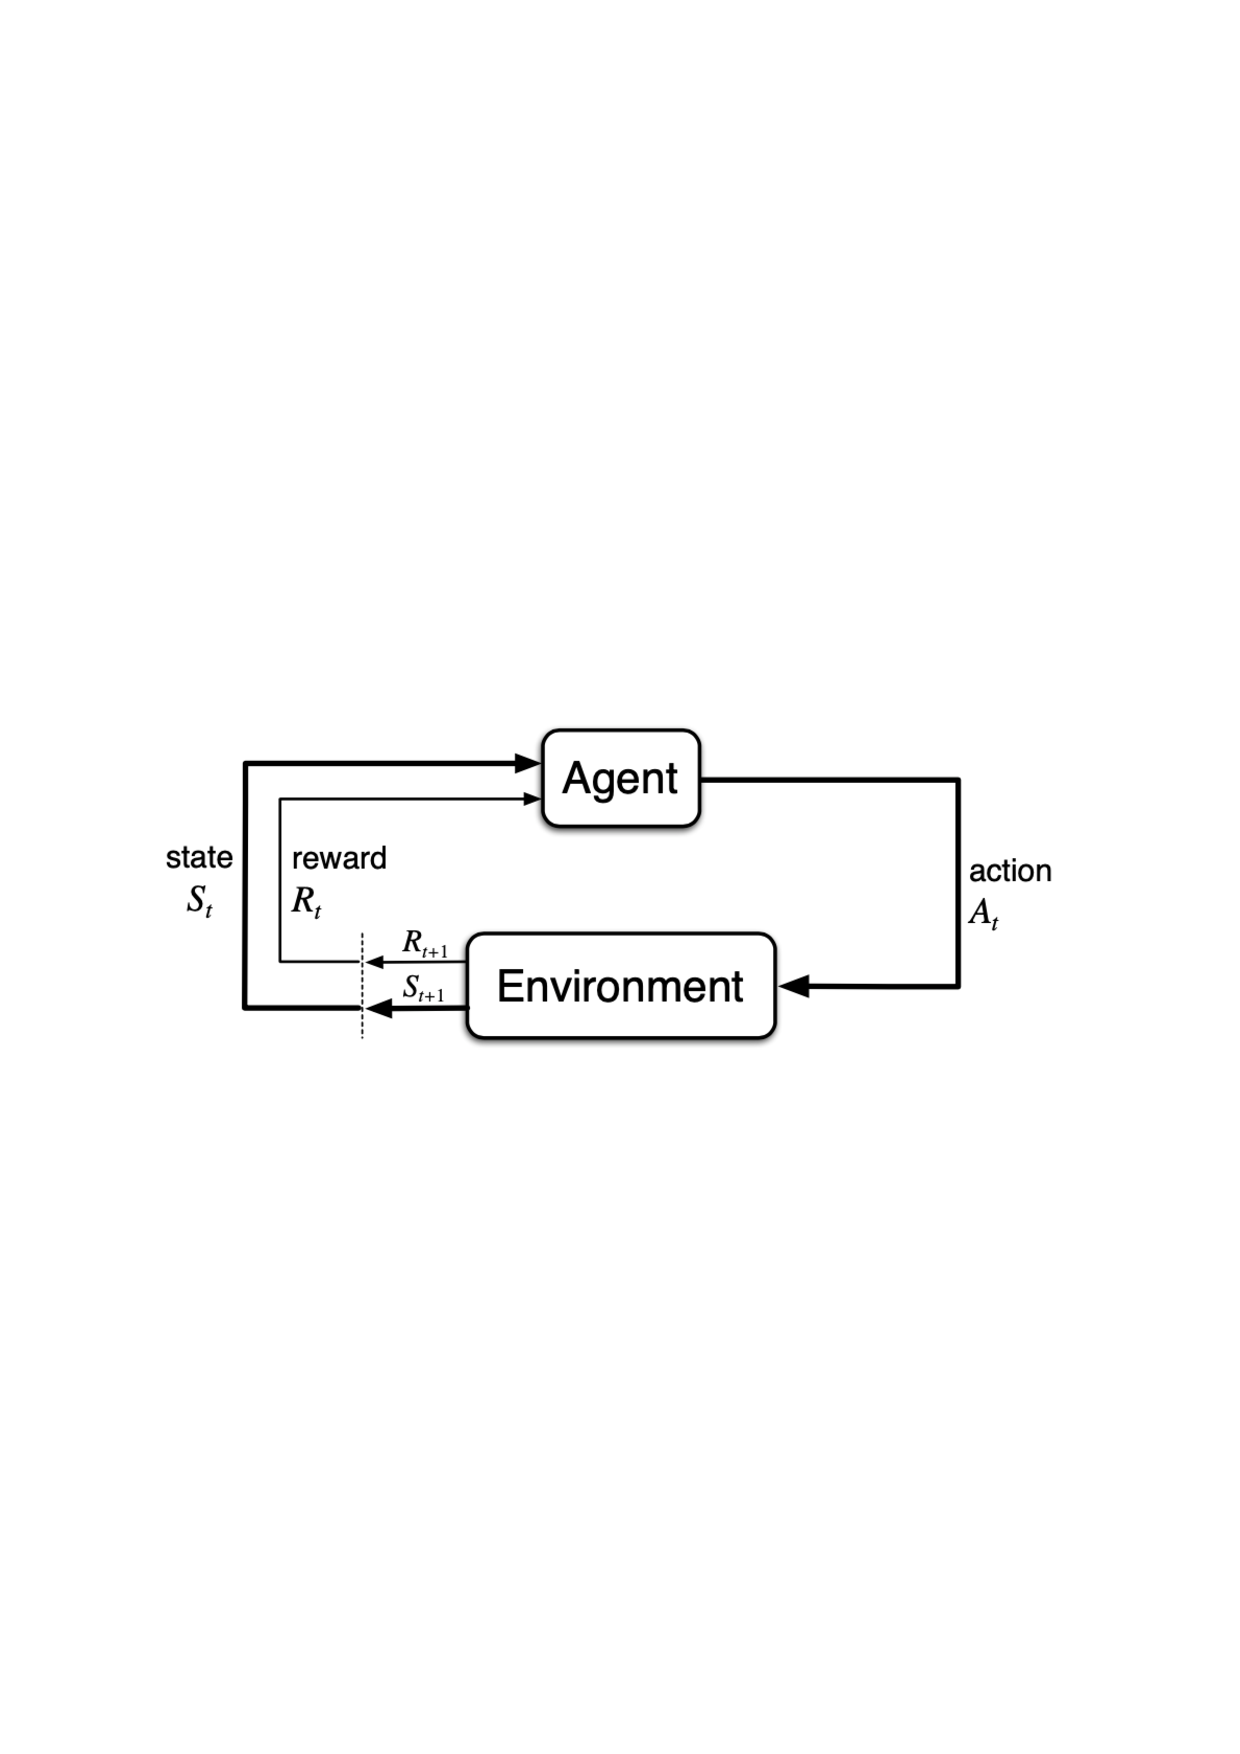
\includegraphics[width=\linewidth{}]{figures/MDP.pdf}
  \caption{MDPの模式図 (文献\cite{Sutton1998}より引用) \label{fig:mdp}}
\end{figure}

2048は有限MDPにそのまま当てはまるゲームである.
すなわち行動集合\textit{A}は上下左右に対応し, 報酬はプレイヤが獲得する得点に対応する.

\subsection{強化学習の目標と価値関数}
一般に強化学習で扱う問題は, エージェントと環境のやり取りが終わる終了状態が存在するepisodic taskと終了状態が存在しないcontinuing taskが存在する. 
episodic taskではエージェントと環境のやり取りを初期状態から終了状態までのエピソードと呼ばれる単位で分割することができる.
\ref{sec:property}節で説明したように2048は必ず終了するゲームであるため, 以降episodic taskでの定義を確認する. 

強化学習の目標は$G_t=\Sigma_{k=0}^T \gamma^k R_{t+k+1}$とすると1エピソードの累積報酬, すなわち$G_0$の期待値を最大化するような方策~(最適方策)~を学習によって見つけることである.
以降$G$をリターンと呼ぶ.
ここで割引率$\gamma$は将来獲得する報酬が現在の状態にどれだけの影響を与えるかを決定する値であり, $\gamma$が0に近づくほどエージェントは現在獲得できる即時報酬を最大化し, 1に近づくほど将来の報酬も考慮するようになる.

状態価値関数$v_{\pi}(s)$は状態$s$から方策$\pi$に従って行動を選択し続けた場合のリターンの期待値であり, 次のように定義される.

\begin{align}
  v_{\pi}(s) \stackrel{\mathrm{def}}{=} \mathbb{E}_{\pi}\left[G_t|S_t=s \right] = \mathbb{E}_{\pi}\left[\sum_{k=0}^T \gamma^k R_{t+k+1}|S_t=s \right]
\end{align}

同様に状態$s$から行動$a$を選択し, その後方策$\pi$に従って行動を選択し続けた場合のリターンの期待値である状態行動価値関数の定義は以下のようになる.
\begin{align}
  q_{\pi}(s,a) \stackrel{\mathrm{def}}{=} \mathbb{E}_{\pi}[G_t|S_t=s, A_t=a] = \mathbb{E}_{\pi}\left[\sum_{k=0}^T \gamma^k R_{t+k+1}|S_t=s, A_t=a \right]
\end{align}

この定義の下で, ある状態$s$の価値とその次の状態$s'$の価値の間の関係は次のベルマン方程式によって記述される.
\begin{align}
  v_{\pi}(s) &= \sum_{a \in A} \pi(a|s) \sum_{s' \in S} p(s'|s,a)[r(s,a,s') + \gamma v_{\pi}(s')] \\
  q_{\pi}(s,a) &= \sum_{s' \in S} p(s'|s,a)\left[r(s,a,s') + \gamma \sum_{a' \in A} \pi(a'|s')q_{\pi}(s',a')\right]
\end{align}
すなわち方策$\pi$に従った際のある状態の価値は, 次の状態の価値と即時報酬の合計を環境のダイナミクスと方策の確率分布で期待値を取ったものである. 
状態行動価値についても同様である.

すでに述べたように, 良い方策とは獲得するリターンの期待値が大きいような方策である.
また状態価値$v_\pi(s)$とは状態$s$から方策$\pi$に従って行動を選択し続けた場合のリターンの期待値である.

よって2つの方策$\pi$と$\pi'$があるとすると, すべての状態$s \in S$について$v_\pi(s) \geq v_{\pi'}(s)$が成り立つならば$\pi$は$\pi'$よりも良い方策だと言える.
ここから最適方策$\pi_*$はすべての方策の中で最も状態価値関数および状態行動価値関数が大きいような方策であると定義できる.

\begin{align}
  \label{eq:v_max}
  v_{\pi_*}(s) &= \max_\pi v_{\pi}(s) \quad \text{for all } s \in S \\
  \label{eq:q_max}
  q_{\pi_*}(s,a) &= \max_\pi q_{\pi}(s, a) \quad \text{for all } s \in S \text{ and } a \in A(s)
\end{align}

さらに式\ref{eq:v_max}, \ref{eq:q_max}から次のベルマン最適方程式を導出することができる.

\begin{align}
  \label{eq:bellman_opt1}
  v_{\pi_*}(s) &= \max_a \sum_{s'}p(s'|s,a)[r(s,a,s') + \gamma v_{\pi_*}(s')] \\
  \label{eq:bellman_opt2}
  q_{\pi_*}(s,a) &= \sum_{s'}p(s'|s,a)[r(s,a,s') +\gamma \max_{a'}q_{\pi_*}(s',a')]
\end{align}

式\ref{eq:bellman_opt1}は最適方策$\pi_*$の下での状態$s$の価値は, すべての行動$a \in A(s)$について$a$を選択した場合の遷移後の状態$s'$の価値と即時報酬の合計を環境のダイナミクスについて期待値を取ったものの最大値であるということを示している.
式\ref{eq:bellman_opt2}も同様に解釈できる.

最適方策の状態価値関数$v_{\pi_*}(s)$, 状態価値関数$q_{\pi_*}(s,a)$をそれぞれ最適状態価値関数, 最適状態行動価値関数という.

\section{2048に対する強化学習の先行研究}